\chapter{计算智能}

\begin{question}
计算智能的含义是什么?它涉及哪些研究分支?
\end{question}
\begin{solution}
计算智能是一种智力方式的低层认知,它取决于制造者提供的数值数据,而不依赖于知识。它与人工智能的主要区别在于它不含知识精品。\par
计算智能涉及神经计算、模糊计算、进化计算和人工生命等领域。
\end{solution}

\begin{question}
试述计算智能(CI)、人工智能(AI)和生物智能(BI)的关系。
\end{question}
\begin{solution}
CI$\subset$AI$\subset$BI;CI与AI的差异要比AI与BI的差异小得多。
\end{solution}

\begin{question}
人工神经网络为什么具有诱人的发展前景和潜在的广泛应用领域?
\end{question}
\begin{solution}
\end{solution}

\begin{question}
简述生物神经元及人工神经网络的结构和主要学习算法。
\end{question}
\begin{solution}
\end{solution}

\begin{question}
考虑一个具有阶梯形阈值函数的神经网络,假设
	\begin{enumerate}
		\item 用一常数乘所有的权值和阈值;
		\item 用一常数加所有的权值和阈值。
	\end{enumerate}
试说明网络性能是否会变化?
\end{question}
\begin{solution}
\end{solution}

\begin{question}
构作一个神经网络,用于计算含有两个输入的XOR函数。指定所用神经网络单元的种类。
\end{question}
\begin{solution}
已知用单层感知机是无法解决XOR问题的,需要增加隐单元。隐单元的数量可以有多种选择。这里给出含有两个隐单元(只有一层隐单元)的前馈神经网络。\par 
	\begin{figure}[h]
		\centering
		\def\layersep{2.5cm}

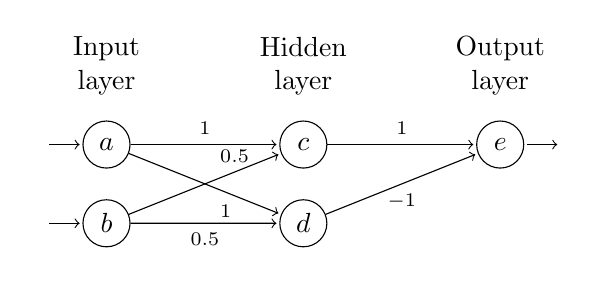
\begin{tikzpicture}[shorten >=1pt,->,draw=black, node distance=\layersep,
	every edge/.append style={nodes={font=\scriptsize}}]
    \tikzstyle{every pin edge}=[<-,shorten <=1pt]
    \tikzstyle{neuron}=[circle,draw=black,minimum size=17pt,inner sep=0pt]
    \tikzstyle{input neuron}=[neuron];
    \tikzstyle{output neuron}=[neuron];
    \tikzstyle{hidden neuron}=[neuron];
    \tikzstyle{annot} = [text width=4em, text centered]

    % Draw the input layer nodes
    %\foreach \name / \y in {1,...,2}
    % This is the same as writing \foreach \name / \y in {1/1,2/2,3/3,4/4}
        \node[input neuron, pin=left:] (I-1) at (0,-1) {$a$};
        \node[input neuron, pin=left:] (I-2) at (0,-2) {$b$};

    % Draw the hidden layer nodes
    %\foreach \name / \y in {1,...,2}
        \node[hidden neuron] (H-1) at (\layersep,-1 cm) {$c$};
        \node[hidden neuron] (H-2) at (\layersep,-2 cm) {$d$};

    % Draw the output layer node
    \path[yshift=0.5cm]
    		node[output neuron,pin={[pin edge={->}]right:}, right of=H-1] (O) {$e$};

    % Connect every node in the input layer with every node in the
    % hidden layer.    
    \path (I-1) edge node[above]{$1$} (H-1);
    \path (I-1) edge node[above=10pt,right=2pt]{$0.5$} (H-2);
    \path (I-2) edge node[below=10pt,right=2pt]{$1$} (H-1);
    \path (I-2) edge node[below]{$0.5$} (H-2);

    % Connect every node in the hidden layer with the output layer
    \path (H-1) edge node[above]{$1$} (O);
    \path (H-2) edge node[below]{$-1$} (O);

    % Annotate the layers
    \node[annot,above of=H-1, node distance=1cm] (hl) {Hidden layer};
    \node[annot,left of=hl] {Input layer};
    \node[annot,right of=hl] {Output layer};
\end{tikzpicture}
		\caption{XOR问题的神经网络} \label{Fig:NN-XOR}
	\end{figure}
支持XOR问题的神经网络可以如图\ref{Fig:NN-XOR}所示。在这个神经网络中,共有5个处理单元,其中,$a$和$b$是输入单元,$c$和$d$是隐单元,它们位于网络的同一层上,$e$是输出单元。各单元的作用函数$O_i = f(a_i)$为阈值型。
\[O_i = \begin{cases}
	1, \quad a_i \geq 1 \\
	0, \quad a_i < 1
\end{cases} \]
\end{solution}

\begin{question}
假定有个具有线性激励函数的神经网络,即对于每个神经元,其输出等于常数$c$乘以各输入加权和。
	\begin{enumerate}
		\item 设该网络有个隐含层。对于给定的权$W$,写出输出层单元的输出值,此值以权$W$和输入层$I$为函数,而对隐含层的输出没有任何明显的叙述。试证明:存在一个不含隐含单位的网络能够计算上述同样的函数。
		\item 对于具有任何隐含层数的网络,重复进行上述计算。从中给出线性激励函数的结论。
	\end{enumerate}
\end{question}
\begin{solution}
\end{solution}

\begin{question}
试实现一个分层前馈神经网络的数据结构,为正向评价和反向传播提供所需信息。应用这个数据结构,写出一个神经网络输出,以作为一个例子,并计算该网络适当的输出值。
\end{question}
\begin{solution}
\end{solution}

\begin{question}
什么是模糊性?它的对立含义是什么?试各举出两个例子加以说明。
\end{question}
\begin{solution}
所谓模糊性是指客观事物在形态及类属方面的不分明性,其根源是在类似食物间存在一系列过渡状态,它们互相渗透,互相贯通,使得彼此之间没有明显的界限。它的对立含义是``确定性''。例如,通常说``某人很年轻''、``某人比较年轻''之间没有明显的界限,所以它们都是模糊的。
\end{solution}

\begin{question}
什么是模糊集合和隶属函数或隶属度?
\end{question}
\begin{solution}
论域$U$到$[0,1]$区间的任意映射$\mu_F$,即$\mu_F \colon U \to [0,1]$,都确定$U$的一个模糊子集$F$,则$\mu_F$称为$F$的隶属函数或隶属度。
\end{solution}

\begin{question}
模糊集合有哪些运算?满足哪些规律?
\end{question}
\begin{solution}
模糊集合的交、并、补。设$A$、$B$是论域$U$上的两个模糊集,分别称$A \cup B$、$A \cap B$为$A$与$B$的并集、交集,称$\overline{A}$为$A$的补集,它们的隶属函数分别为:
	\begin{align*}
		\mu_{A \cup B}(u) &= \max \left\{ \mu_A(u), \mu_B(u) \right\} \\
		\mu_{A \cap B}(u) &= \min \left\{ \mu_A(u), \mu_B(u) \right\} \\
		\mu_{\overline{A}} &= 1 - \mu_A(u)
	\end{align*}
\end{solution}

\begin{question}
什么是模糊推理?
\end{question}
\begin{solution}
模糊推理以模糊判断为前提,动用模糊语言规则,推导出一个近似的模糊判断理论。
\end{solution}

\begin{question}
对某种产品的质量进行抽查评估。现随机选出5个产品$x_1$,$x_2$,$x_3$,$x_4$,$x_5$进行检验,它们质量情况分别为:
\[ x_1=80, x_2=72, x_3=65, x_4=98, x_5=53\]
这就确定了一个模糊集合$Q$,表示该组产品的``质量水平''这个模糊概念的隶属程度。
试写出该模糊集。
\end{question}
\begin{solution}
该模糊集为$Q={(x_1,0.8), (x_2, 0.72), (x_3,0.65), (x_4,0.98), (x_5,0.53)}$。
\end{solution}

\begin{question}
试述遗传算法的基本原理,并说明遗传算法的求解步骤。
\end{question}
\begin{solution}
遗传算法的基本原理是,通过随机方式产生若干个所求解问题的数字编码,即染色体,形成初始种群;通过适应度函给每个个体一个数值评价,淘汰低适应度的个体,选择高适应度的个体参加遗传操作,经过遗传操作后的个体集合形成下一代新的种群。再对这个新的种群进行下一轮的进化。\par
遗传算法的求解步骤:\par
	\begin{enumerate}
		\item 初始化种群;
		\item 计算种群上每个个体的适应度值;
		\item 按由个体适应度值所决定的某个规则选择将进入下一代的个体;
		\item 按概率$P_c$进行交叉操作;
		\item 按概率$P_c$进行变异操作;
		\item 若没有满足某中停止条件,则转(2),否则进入下一步;
		\item 输出中群中适应度最优的染色体作为问题的满意解或最优解。
	\end{enumerate}
\end{solution}

\begin{question}
如何利用遗传算法求解问题,试举例说明求解过程。
\end{question}
\begin{solution}
\end{solution}

\begin{question}
用遗传算法求$f(x)=x\cos x + 2$的最大值。
\end{question}
\begin{solution}
\end{solution}

\begin{question}
什么是人工生命?请按你的理解用自己的语言给人工生命下个定义。
\end{question}
\begin{solution}
具有自然生命现象和(或)特征的人造系统,都可称为人工生命。
\end{solution}

\begin{question}
人工生命要模仿自然生命的特征和现象。自然生命有哪些共同特征?
\end{question}
\begin{solution}
自然生命的共同特征和现象包括但不限于:
	\begin{enumerate}
		\item 自繁殖、自进化、自寻优;
		\item 自成长、自学习、自组织;
		\item 自稳定、自适应、自协调;
		\item 物质构造;
		\item 能量转换;
		\item 信息处理。
	\end{enumerate}
\end{solution}

\begin{question}
为什么要研究人工生命?
\end{question}
\begin{solution}
研究和开发人工生命,有利于
	\begin{enumerate}
		\item 开发基于人工生命的工程技术新方法、新系统、新产品;
		\item 为自然生命的研究提供新模型、新工具、新环境;
		\item 延伸人类寿命、减缓衰老、预防疾病;
		\item 扩展自然生命,实现人工进化和优生优育;
		\item 促进生命科学、信息科学、系统科学的交叉与发展。
	\end{enumerate}
	因此,人工生命的研究开发及应用具有重大的科学意义、广泛的应用前景、深远的社会影响、以及显著的经济效益。
\end{solution}

\begin{question}
人工生命包括哪些研究内容?其研究方法如何?
\end{question}
\begin{solution}
人工生命的研究内容大致可分为两类:
	\begin{enumerate}
		\item 构成生物体的内部系统,包括脑、神经系统、内分泌系统、免疫系统、遗传系统、酶系统、代谢系统等。
		\item 生物体及其群体的外部系统,包括环境适应系统和遗传进化系统等。
	\end{enumerate} \par
	人工生命的研究方法主要可分为两类:
	\begin{enumerate}
		\item 信息模拟法。根据内部和外部系统所表现的生命行为来创造信息模型。
		\item 工作原理法。生命行为所显示的自律分散和非线性行为,其工作原理是混沌和分形,以此为基础研究人工生命的机理。
	\end{enumerate}
\end{solution}